\section{研究方法、技术路线、实验方案}

\subsection{研究方法}
\begin{frame}{\insertsection}{\insertsubsection}
	\begin{center}
		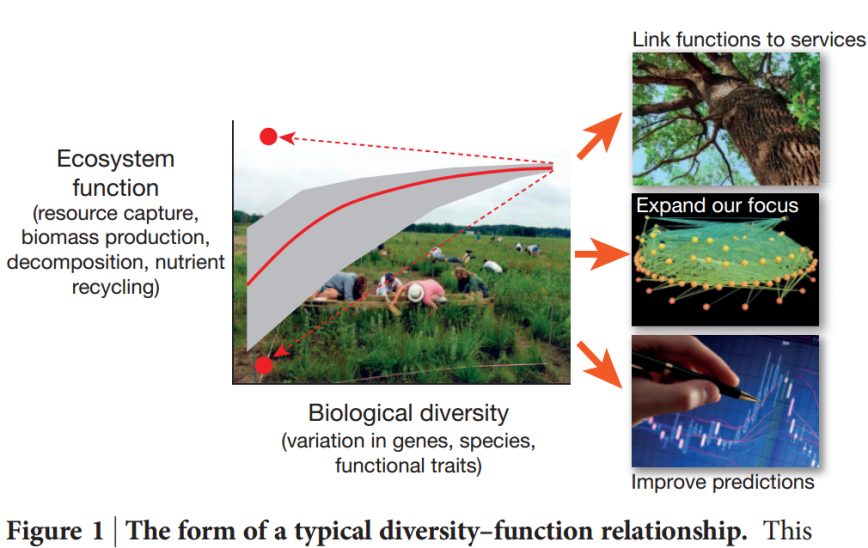
\includegraphics[width = 0.9\textwidth]{./pic/2.1.png}
	\end{center}
1)植物多样性梯度;
2)土壤微生物多样性梯度;\\
3)演替梯度;
4)环境因子梯度;\\
5)功能群移除;
\end{frame}
\begin{frame}{\insertsection}{\insertsubsection}
研究地点:
西藏、青海、内蒙古南北两条平行样带
	\begin{center}
		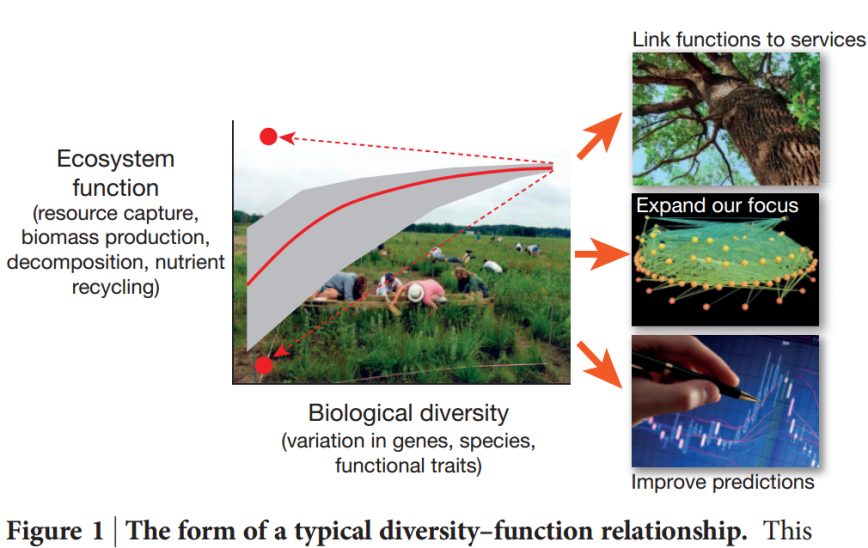
\includegraphics[width = 0.9\textwidth]{./pic/2.1.png}
	\end{center}
\end{frame}



\begin{frame}{\insertsection}{\insertsubsection}
	研究地点:
	于生长季顶期分别从西藏、青海、内蒙三个省份,沿从东到西的水分梯度分成南、北两条平行样带进行采样。记录每个样点的植被类型和温度,并用GPS记录每个样点的地理坐标和海拔。
\end{frame}
\subsection{技术路线}
\begin{frame}{\insertsection}{\insertsubsection}
	\begin{center}
		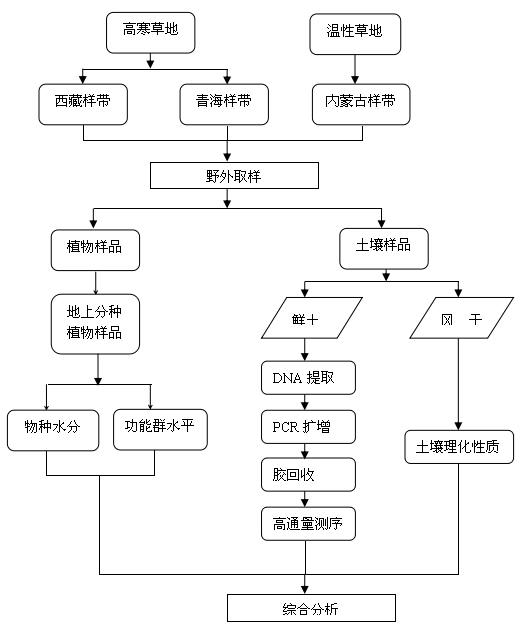
\includegraphics[width = 0.6\textwidth]{./pic/技术路线.jpg}
	\end{center}
\end{frame}
\subsection{实验方案}
\begin{frame}{\insertsection}{\insertsubsection}
	\begin{center}
		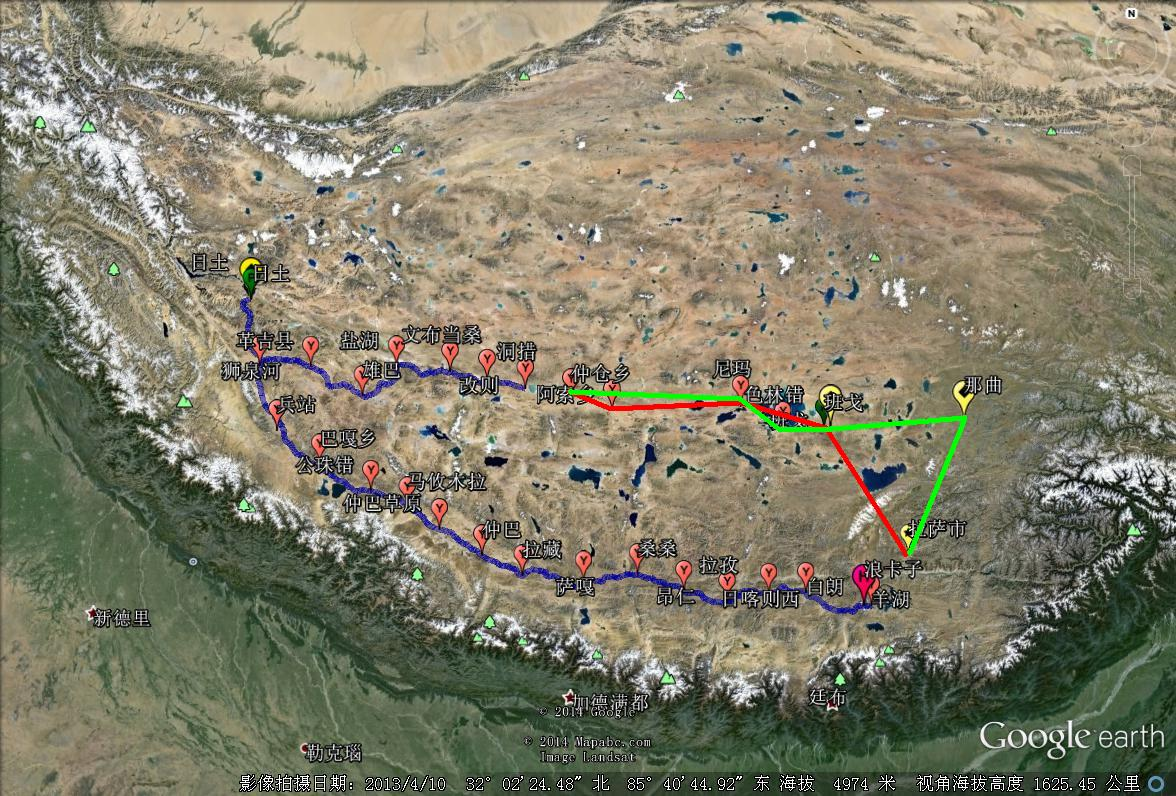
\includegraphics[width = 0.9\textwidth]{./pic/西藏瓦岗.jpg}
	\end{center}
	1)在西藏冈底斯山脉南北两侧,沿水分梯度各由东往西定点取样;
\end{frame}

\begin{frame}{\insertsection}{\insertsubsection}	
	\begin{columns}
		\column{0.5\textwidth}
		\begin{center}
			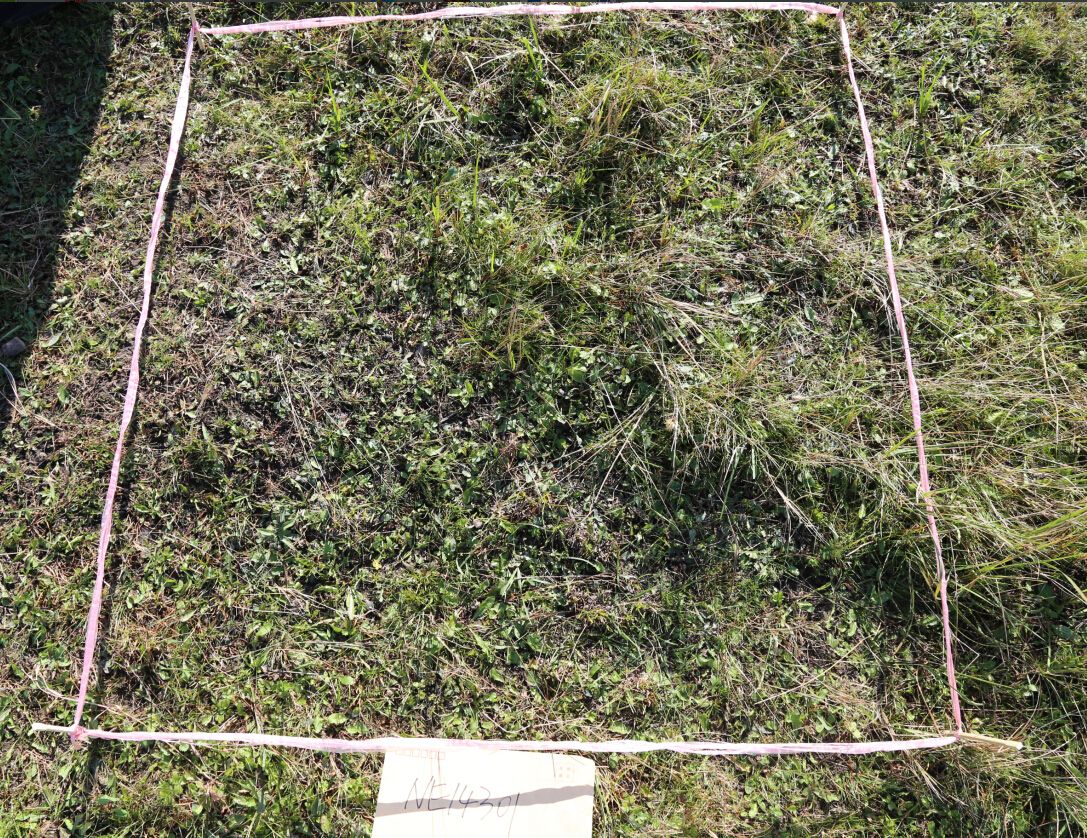
\includegraphics[width = 1.1\textwidth]{./pic/2.2.1.jpg}
		\end{center}		
		\column{0.5\textwidth}
		\begin{center}
			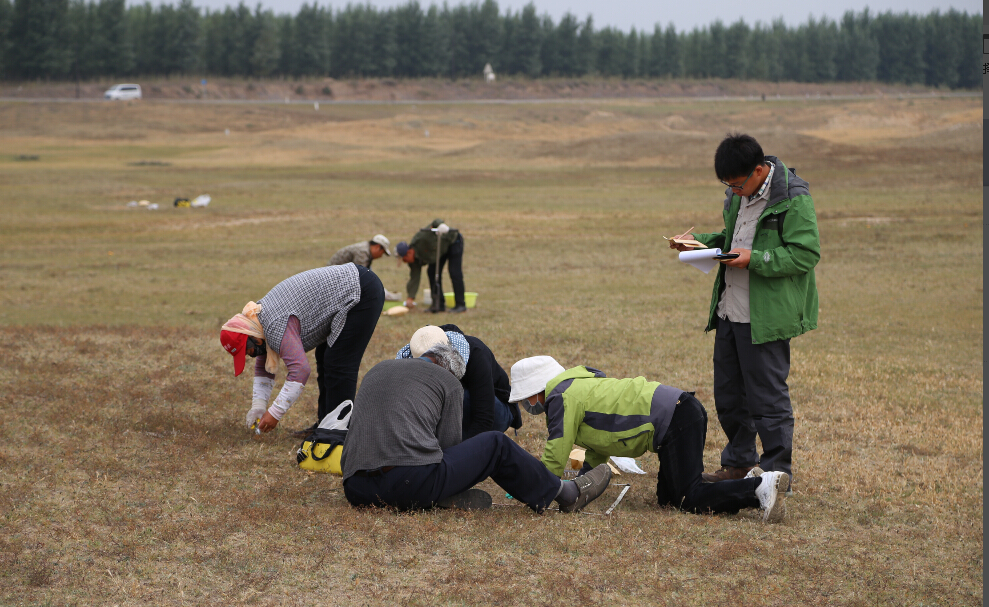
\includegraphics[width = 1.4\textwidth]{./pic/2.2.2.jpg}
		\end{center}
	\end{columns}
	\vskip 2em
	2)在每个取样点,随机选择5个1m×1m的样方,记录每个物种(随机选取5株)的高度,分种剪取地上植物生物量,称鲜重,实验室65℃烘72小时,称干重;	
\end{frame}
\begin{frame}{\insertsection}{\insertsubsection}	
	\begin{columns}
		\column{0.5\textwidth}
		\begin{center}
			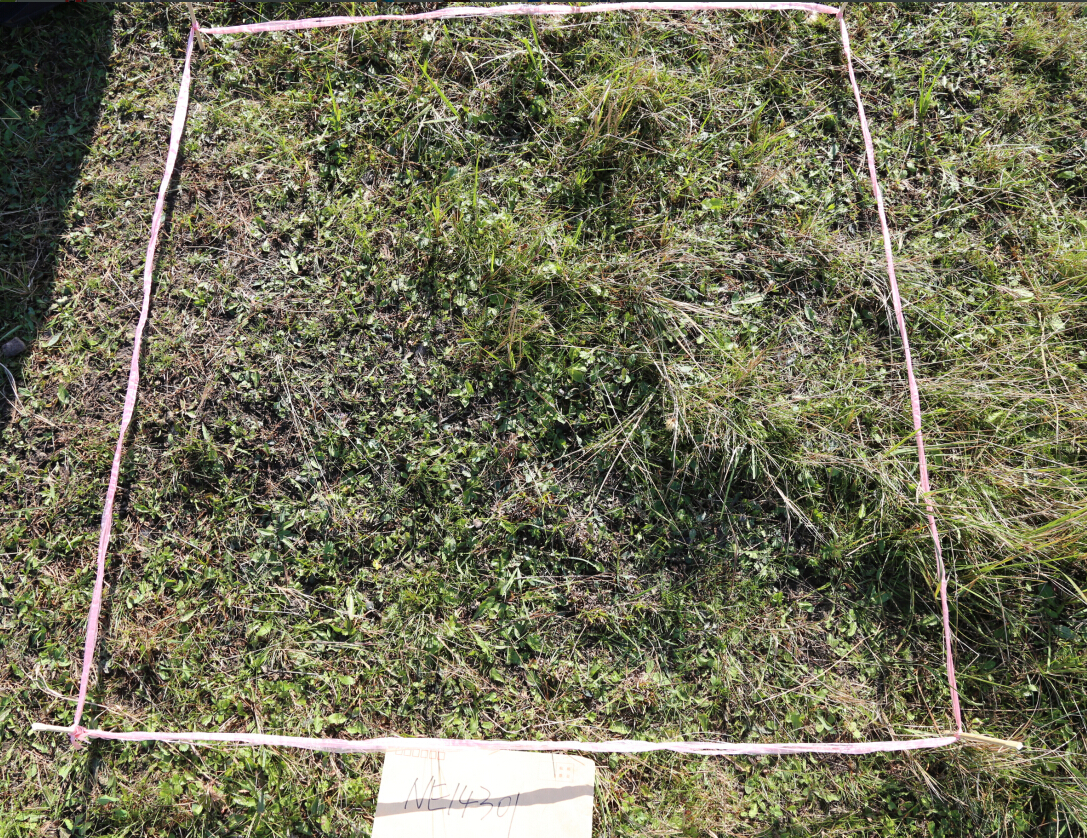
\includegraphics[width = 1.1\textwidth]{./pic/2.3.1.jpg}
		\end{center}		
		\column{0.5\textwidth}	
		\begin{center}
			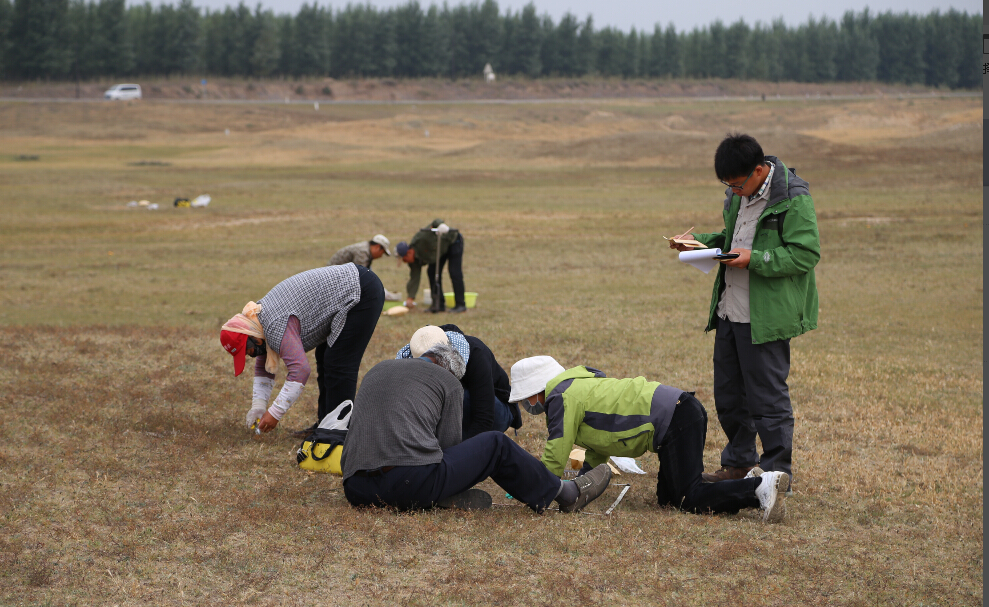
\includegraphics[width = 1.05\textwidth]{./pic/2.3.2.jpg}
		\end{center}
	\end{columns}
	\vskip 2em
	3)在每个取样点随即选择的5个1m×1m的样方剪除地上生物量后,用5cm根钻每层(0-10cm、10-20cm、20-30cm)取3钻土壤样品并均匀混合,一半土壤样品迅速放入野外冰箱并冷冻保存,用于提取微生物DNA;另外一半带回实验室风干,用于测量土壤的理化性质;	
\end{frame}

\begin{frame}{\insertsection}{\insertsubsection}
4)利用风干土壤样品测定土壤的主要理化性质指标;
5)利用冷冻保存的土壤样品提取微生物DNA、扩增16S rRNA、凝胶回收、高通量测序;
6)根据地上分钟植物样品计算各样方物种的丰富度、多度、多样性,按照功能群分类计算各样方功能群的多样性,并分析在沿水分梯度条件下它们与土壤微生物多样性的关系;
\end{frame}


